\documentclass[a4paper,12pt]{article}
\usepackage{graphicx}
\usepackage{caption}
\usepackage{subcaption}
\usepackage{float}
\usepackage[margin=1in]{geometry}
\usepackage{lmodern}
\usepackage{amsmath}
\usepackage{xcolor}
\usepackage{listings}
\usepackage{pgffor}

\begin{document}

\title{Relatório Bayes 2}
\author{Eduardo}
\date{\today}
\maketitle

\begin{figure}[H]
    \centering
    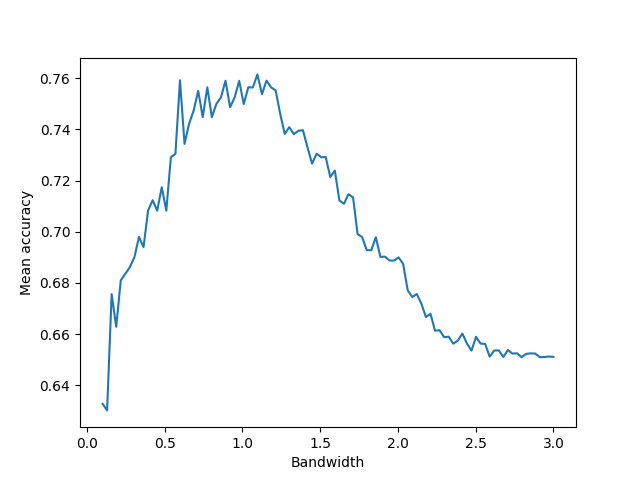
\includegraphics[width=0.8\textwidth]{accuracy_vs_bandwidth.png}
    \caption{Accuracy vs Bandwidth}
    \label{fig:accuracy_vs_bandwidth}
\end{figure}

Max accuracy is achieved with a bandwidth of approximately 1.0.

\begin{figure}[H]
    \centering
    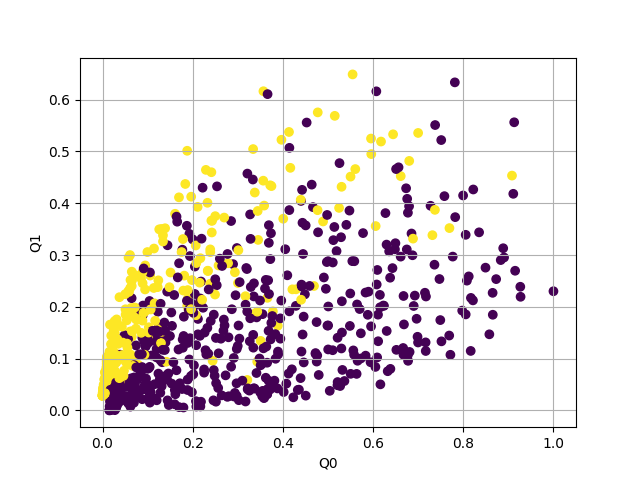
\includegraphics[width=0.8\textwidth]{best_h.png}
    \caption{Best h=0.98}
    \label{fig:best_h}
\end{figure}

Visualy, the best accuracy is achieved when the samples are uniformly distributed in the likelihood space, with some overlap between the classes.

\begin{figure}[H]
    \centering
    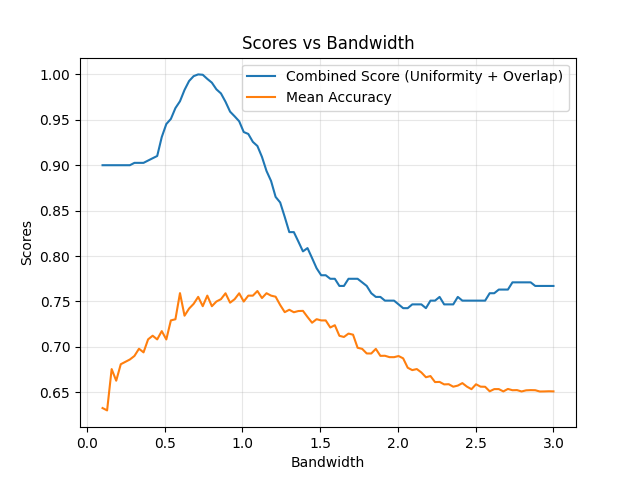
\includegraphics[width=0.8\textwidth]{scores_vs_bandwidth.png}
    \caption{Combined Score vs Bandwidth}
    \label{fig:scores_vs_bandwidth}
\end{figure}

The combined score is defined as a weighted linear combination of two components: the uniformity score and the overlap score. Let $S_{\text{uniformity}}$ represent the uniformity score and $S_{\text{overlap}}$ represent the overlap score. The combined score $S_{\text{combined}}$ is given by:

\[
S_{\text{combined}} = w_{\text{uniformity}} S_{\text{uniformity}} + w_{\text{overlap}} S_{\text{overlap}},
\]

where $w_{\text{uniformity}}$ and $w_{\text{overlap}}$ are the weights assigned to the uniformity and overlap scores, respectively, such that $w_{\text{uniformity}} + w_{\text{overlap}} = 1$.

The uniformity score $S_{\text{uniformity}}$ measures how evenly the samples are distributed within their respective regions in the likelihood space. It is computed as the proportion of non-empty bins in a discretized triangular region for each class, averaged over all classes:

\[
S_{\text{uniformity}} = \frac{1}{2} \left( \frac{\text{Non-empty bins in Region 0}}{\text{Total bins in Region 0}} + \frac{\text{Non-empty bins in Region 1}}{\text{Total bins in Region 1}} \right).
\]

The overlap score $S_{\text{overlap}}$ quantifies the degree of overlap between the two classes in the likelihood space. It is defined as:

\[
S_{\text{overlap}} = 1 - \frac{\left| O_{\text{actual}} - O_{\text{desired}} \right|}{O_{\text{desired}}},
\]

where $O_{\text{actual}}$ is the observed overlap proportion, $O_{\text{desired}}$ is the desired overlap proportion, and the score is clipped to the range $[0, 1]$.

The combined score $S_{\text{combined}}$ is designed to balance the trade-off between uniformity and overlap, with the weights $w_{\text{uniformity}}$ and $w_{\text{overlap}}$ controlling the relative importance of these two factors. Empirically, it has been observed that $S_{\text{combined}}$ correlates well with classification accuracy, making it a reliable predictor for model performance.

\end{document}
